
\chapter{Implementation and Evaluation}
\label{chap:implementation}

In section \ref{sec:challenges} we presented the three main challenges of this research paper: portability, security and speed. To accurately assess whether the design presented in chapter \ref{chap:solution} meets these challenges, an example system was implemented by the researchers of this paper. The first part of chapter is devoted to illustrating the various aspects of this implementation. In the second part of this chapter, this implementation is evaluated and analysed with regard to the challenges proposed earlier. 

\section{Implementation}
The structure of this section is as follows: First, the individual pieces of hardware that were used in the implementation are discussed. Second, the set-up of the demo in general is explained. In the last section of this chapter, the implementations of the three key aspects of section \ref{sec:obd2_access_control} are illustrated (authenticated key agreement procedure, message authentication procedure and permissions table).

\subsection{Hardware}
\label{sec:hardware}
It is clear that the design presented in chapter \ref{chap:solution}, as well as the OBD-II system is general, is of an embedded nature. The gateway ECU is embedded by default, since it is implemented by a microcontroller in all extant intra vehicle networks. The tester device however, introduced by the researchers of this paper, could be either implemented by an embedded device (e.g. tester), or a software application running on a standard PC (e.g. a laptop owned by the repair shop), that is connected to the OBD-II port via some adapter. The decision was made to implement the former (i.e. the tester is also embedded). Because of this decision, the tester and gateway can be implemented on the same microcontroller architecture. This also means that the same CAN messaging library can be used in both microcontrollers.\\ \\ The goal of this implementation is to serve as a proof of the practical feasibility of our proposed solution. This is why the choice of hardware architecture is very important. The idea is that if an implementation on a resource constrained microcontroller, would meet our challenges (i.e. portability, security and speed). This would prove that implementation is possible on all microcontrollers that feature better specifications than the one we used in our demo. This is why we chose to select a microcontroller architecture that is as limited as possible.  \\ \\ The microcontroller chosen for our implementation is the Atmel AT90CAN128. Which has a word size of 8 bits, boasts a 128 KB flash memory, 4KB of EEPROM and 4KB SRAM (for more information on these specifications see  Section \ref{sec:microcontrollers}). More importantly, it includes a dedicated CAN controller, which allows for easy CAN networking between devices. The DVK90CAN1 is a development kit that includes the AT90CAN128, as well as introducing a series of hardware peripherals like power supply inputs,LEDS, buttons, connectors, transceivers, programming interfaces, debuggers, etc. The ones that were extensively used in our implementation are:
\begin{itemize}
	\item \textbf{Programming/Debugging interface:} The DVK90CAN1 includes the option of easily connecting to a standard PC for programming and debugging. This is done by connecting the ATMEL-ICE BASIC programmer to both the DVK90CAN1 board and a PC running Atmel Studio, which is an integrated development platform (IDP) that allows us to run and debug C and assembly code on both microcontrollers.
	
	\item \textbf{CAN Transceiver:} This device functions as a transmitter and receiver by transmitting messages from the CAN controller on to the CAN bus (male DB9), as well as receiving incoming CAN messages and forwarding them to the CAN controller. 
	
	\item \textbf{Male DB9:} This connector belongs to the D-sub series, where the B denotes the shell size and the 9 means there are 9 pins. This connector assumes the CAN bus connections.
	
	\item \textbf{RS-232 driver/receiver:} Recommended standard 232 (RS-232) is a standard for serial transmission of data. The driver/receiver is responsible for transmitting and receiving RS-232 data (female DB-9).
	
	\item \textbf{Female DB9:} This connector assumes the RS-232 connections.
	
	\item \textbf{Compass Card Keyboard} 4 de-centered push-buttons of compass card keyboard are present on the board, allowing for user interactivity.
\end{itemize}
Besides some peripherals offered by the DVK90CAN1 board and the ATMEL-ICE BASIC programmer, two more pieces of hardware were use in our system. First; there's a female-to-female DB9 cable. This is used to connect the CAN interfaces of both boards. Second there's a male-to-male DB9 cable that is connected to a generic RS232 to USB converter. This cable allows both boards to be connected to a PC for serial communications.

\subsection{Demo Set-Up}
\label{sec:demo_setup}

Figure \ref{fig:demo} shows the set-up of the implementation. One board functions as the tester, which is connected via CAN (using the female-to-female DB9 cable) to the other board, which in turn functions as the gateway. This connection is used to implement the general authenticated key agreement and message authentication procedures presented in Section \ref{subsec:authenticated_key_agreement_procedure} and \ref{subsec:message_authentication_procedure}. The permission table outlined in Section \ref{subsec:sol_permissions_table} is implemented on the gateway. The gateway is also connected to a PC using the RS-232 communications standard, to allow for real time feedback (e.g. signalling when a signature verification procedure successfully terminates). The attentive reader might notice two integral components missing from this set-up: the central server that is introduced in Section \ref{fig:authentication_procedure}, as well as the intra vehicle network itself. The decision was made to implement these components only logically. This was done for two reasons: first, a realistic implementation of these components would result in the introduction of more hardware, greatly increasing the time and cost required to construct a working demo. Second, since the primary focus of this paper is the RBAC system proposed in chapter \ref{chap:solution}, as well as all the procedures and systems introduced to enforce it on the gateway (i.e. authenticated key agreement procedure, message authentication procedure and permissions table); providing a physical central server and intra vehicle network implementation can be considered out of scope. The logical implementation of both these components was done as follows:
\begin{itemize}
	\item \textbf{Central Server:} The software on the tester board implements a dedicated key-API that specifies a series of private key related functions (for signing and calculating the shared secret). As far as the main tester software is concerned, calling these functions could result in a remote server being addressed.
	
	\item \textbf{Intra Vehicle Network:} The RS-232 connection between gateway and PC is used for this purpose. Whenever a message is accepted by the gateway, instead of forwarding the message to another sub-network, a message is transmitted to the PC. This message contains the ID of the accepted message, as well as a line of text signalling that the message was accepted.
\end{itemize}

\begin{figure}[h]
	\label{fig:demo}
	\caption{Hardware set-up that is used to implement the proposed solution.}
\end{figure}

\subsection{OBD-II Access Control Implementation}
The key aspects aspects of the OBD-II access control system presented in chapter \ref{chap:solution} are the authenticated key agreement procedure, the message authentication procedure and of course the permissions table. How these were implemented in the set-up presented in Section \ref{sec:demo_setup} is discussed next. 

\subsubsection{Authenticated Key Agreement Procedure Implementation}
\label{subsec:authenticated_key_agreement_procedure_implementation}

Figure \ref{fig:authentication_procedure_implementation} shows how the authentication procedure was implemented in our demo. Because of our decision to omit the central server and the intra vehicle network, these are naturally not included in the diagram. Because of this, the tester now stores the OBD-II private key $P_{obd}$ instead of the central server. In our diagram we have chosen to include the size of this key (in bits) in the superscript: $Pr_{obd}^{256}$. This was repeated for every piece of data in the diagram (e.g. keys and signatures). The corresponding public key $Pb_{obd}^{512}$ is stored on the gateway. The size of these keys was mandated by the decision to guarantee a security level of 128 bits (see \ref{sec:security_level}). As mentioned in Section \ref{subsec:ECC}, the decision was made to use elliptic curve asymmetric key pairs. The TinyECC\footnote{\url{https://github.com/kmackay/micro-ecc}} C library offers a safe and efficient implementation for ECC operations on AVR microcontrollers. According to \cite{Siddiqui}, ECC keys have the property that the size of the underlying field (i.e. the size of the key), should be twice the security parameter. The decision was made to work with the secp256r1 curve (also supported by TinyECC), which meets our security level guarantee ($\frac{256}{2}=128$) and introduces fixed sizes for our keys (256 bit for the private key and 512 bits for the public key).

\paragraph{The Procedure}

The authentication procedure is initiated by the tester, which transmits an initialisation message to the gateway. This message contains the role that the tester wishes to authenticate as: $Role^8$. Because it is only 8 bits in size, it fits into a single CAN message (remember from Section \ref{subsec:can:frames}, Figure \ref{fig:CANframe} that a CAN message can hold up to 64 bits of data). The gateway reacts to this message by creating a new ECC keypair: KGen($Pb_g^{512}$,$Pr_g^{256}$. The same curve must be used as the one chosen for the original OBD-II keys (i.e. secp256r1), otherwise the ECDH secret generation algorithm used later on won't work. As a result of this, both key pairs have the same respective sizes. Next, the newly generated public key $Pb_g^{512}$ is transmitted to the tester. Because of it's size (512 bits), this key won't fit into a single CAN message. This problem is overcome by spreading the key over 8 distinct CAN messages, and sending them to the tester one by one. After the tester receives all 8 messages, and assembles the public key, it will first hash it using SHA512: SHA512($Pb_g^{512}$). For this operation the AVR cryptolib\footnote{\url{https://github.com/cantora/avr-crypto-lib}} C library was chosen. After calculating the hash value, the signing function of the key API is called: Sig(SHA512($Pb_g^{512}$),$Pr_{obd}^{256}$). This results in the signature being generated: $S^{512}$. The size of our signature is determined by our choice of curve; Our curve corresponds to a signature size of 512 bits. Once the signature is generated, it sent to the gateway. Because the signature is the same size as the public key that was sent earlier, it is also spread over 8 different CAN messages. Upon reception, the gateway verifies the validity of the signature by first hashing it with the same hash function used in it's generation (SHA512), before running the ECDSA verification procedure: Ver(SHA512($S^{512}$),$Pb_{obd}^{512}$). If and when the verification is successful, an ACK message is transmitted to the tester. Both tester and gateway can now generate the shared secret: ECDH($Pr_{obd}^{256}$,$Pb_g^{512}$) and ECDH($Pr_g^{256}$,$Pb_{obd}^{512}$), which will be used in the message authentication procedure.

\begin{figure}[h]
	\centering
	\fbox{
		\procedure{OBD-II authenticated key agreement procedure implementation}{%
			\textbf{Tester}  \<\< \textbf{Gateway} \\
			\text{$Pr_{obd}^{256}$} \<\< \text{$Pb_{obd}^{512}$} \\
			\< \sendmessageright{top=\text{$Role^8$ (1 frame)}} \<\\
			\<\< \text{KGen($Pb_g^{512}$,$Pr_g^{256}$)} \\
			\< \sendmessageleft{top=\text{$Pb_g^{512}$ (8 frames)}} \<\\
			\text{$S^{512}$=Sig(SHA512($Pb_g^{512}$),$Pr_{obd}^{256}$)} \<\<\<\< \\
			\< \sendmessageright{top=\text{$S^{512}$ (8 frames)}} \<\\
			\<\< \text{Ver(SHA512($S^{512}$),$Pb_{obd}^{512}$)} \\
			\< \sendmessageleft{top=\text{$ACK^{8}$ (1 frame)}} \<\\
			\text{$K^{256}$=ECDH($Pr_{obd}^{256}$,$Pb_g^{512}$)} \<\< \text{$K^{256}$=ECDH($Pr_g^{256}$,$Pb_{obd}^{512}$)} \\
		}
	}
	\caption{OBD-II authenticated key agreement procedure implementation}
	\label{fig:authentication_procedure_implementation}
\end{figure}



\subsubsection{Message Authentication Procedure Implementation}
\label{subsec:message_authentication_procedure_implementation}

Figure \ref{fig:message_authentication_implementation} shows the implementation of the message authentication procedure. After the procedure from section \ref{subsec:authenticated_key_agreement_procedure_implementation} completes, and the shared secret $K$ is established, this procedure is repeated for every OBD-II message sent by the tester. The procedure starts when the tester sends the message $M^{64}$ (again superscript is used to indicate the size). The gateway receives the message and checks the permissions table: CheckP($M^{64}$(see section \ref{subsec:permissions_table_implementation}), before sending an acknowledgement back to the tester: $ACK^8$. This acknowledgement is positive or negative based on the outcome of the earlier permissions table check. Upon reception of the acknowledgement, the tester calculates the MAC of the message using the shared secret and HMAC\textunderscore SHA256: $Mac^{256}$=Hmac\textunderscore SHA256($M$,$K$)\footnote{To reduce the performance overhead, the MAC can be computed right after sending the original OBD-II message. This would allow the MAC to be ready before the first acknowledgement is received.}. For the HMAC\textunderscore SHA256 operation the AVR cryptolib library is used, just like we did for SHA512 in section \ref{subsec:authenticated_key_agreement_procedure_implementation}. The size of this MAC is again mandated by our security guarantee of 128 bits. This is because the SHA265 cryptographic hash algorithm has a security level of 128 bits against collision attacks. The MAC is then sent to the Gateway, which will in turn verify it using the shared secret: Ver($Mac^{256}$,$K$). If the MAC is valid, the original message $M^{64}$ is forwarded to the intra vehicle network: Forward($M^{64}$), which in our implementation was indicated by sending a RS232 message to a connected PC. The tester is also informed of this by sending another acknowledgement. Upon reception the tester might want to send another message, in which case the entire procedure is repeated. 

\begin{figure}[h]
	\centering
	\fbox{
		\procedure{Message Authentication}{%
			\textbf{Tester}  \<\< \textbf{Gateway} \\
			\text{$K$}  \<\< \text{$K$} \\
			\< \sendmessageright{top=\text{OBD-II message $M^{64}$ (1 frame)}} \<\\
			\<\< \text{CheckP($M^{256}$)} \\
			\< \sendmessageleft{top=\text{$ACK^8$ (1 frame)}} \< \\
			\text{$Mac^{256}$=Hmac\textunderscore SHA256($M$,$K$) } \<\< \\
			\< \sendmessageright{top=\text{$Mac^{256}$} (4 frames)} \<\\
			\<\< \text{Ver($Mac^{256}$,$K$)}  \\
			\<\< \text{Forward($M^{64}$)}  \\
			\< \sendmessageleft{top=\text{$ACK^8$ (1 frame)}} \< \\
		}
	}
	\caption{OBD-II Message Authentication Implementation}
	\label{fig:message_authentication_implementation}
\end{figure}

\subsubsection{Permissions Table Implementation}
\label{subsec:permissions_table_implementation}

The permissions table is implemented according to the design of Section \ref{subsec:permissions_table}. Generally, a permissions table for a RBAC system will use hash functions to map user names to fixed size indices. However, in our case the user names are replaced by CAN message ID's, which already have a fixed size of 11 bits (or 29 if the extended frame format is used), negating the need for any hash functions. Table \ref{table:permissions} shows how the permission table was implemented. The upper table lists all the roles currently implemented, as well as their byte representation (This byte representation is also used in the $Role^{8}$ message of the authentication procedure in section \ref{subsec:authenticated_key_agreement_procedure_implementation}). Beneath this, the implementation of the example of table \ref{table:2} is given. Every ID entry points to a data structure consisting of a series of bytes; each one associated with a role. The presence of a certain role in this series of bytes, indicates that this role has the permission to send a message with the aforementioned ID. Permissions are easily granted and revoked (Admin role) by deleting and adding role bytes to the data structure pointed to by the chosen ID. 

\begin{table}[h]
	\label{table:permissions}
	\centering
	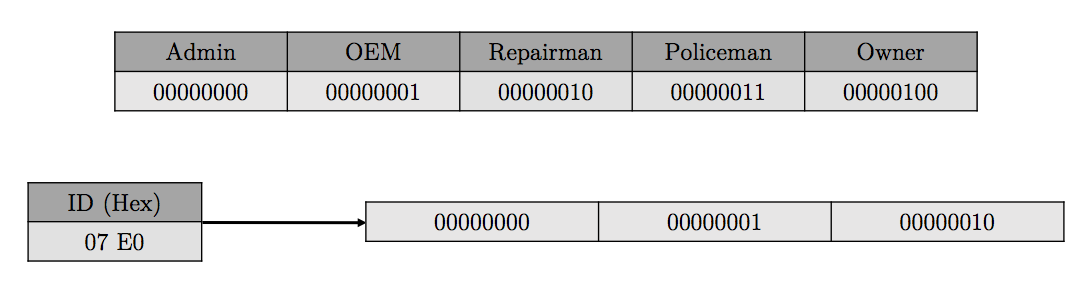
\includegraphics[width=\textwidth]{permissions.png}
	\caption{Permissions table implementation with example.}
\end{table}


\section{Evaluation}
\label{chap:evaluation}

As mentioned in section \ref{sec:challenges}, the main challenge of this research topic are the portability, security and speed of the proposed system, namely the OBD-II access control system that is introduced in chapter \ref{chap:solution}. After introducing the demo implementation in section \ref{chap:implementation}, it is time to assess whether it meets the aforementioned challenges; proving the feasibility it's design. This chapter is structured according to our three challenges. First, the overall portability of the system is quantified, by looking at the memory footprint of the software that is deployed on our gateway microcontroller. Second, the overall security is determined by surveying any potential vulnerabilities. Third, we look at the speed it takes to perform the various procedures. In the last part of this chapter we will gather all the results to conclude whether all of our challenges are met.   

\subsection{Portability}
\label{sec:portability}

The portability of our system refers to the ease at which it is introduced in extant vehicle networks. A system that consists of introducing specific hardware, requiring lots of modifications to be made to the vehicle, is unsuitable. Our system consists of introducing additional code to the gateway. In theory, this would consists of simply reprogramming the gateway microcontroller. Granted, the size of the code that enforces the access control system, is bounded by the memory specifications of the gateway. This is why the size of the code that is introduced to the gateway should be kept as small as possible. As an indication, we can take a look at the size of the code of our demo. 

TODO: discuss memory.

Once the OBD-II system is introduced to a vehicle's gateway ECU, no additional modifications are required to the vehicle. However, there are two more elements required too arrive at a fully functional system: the tester and the central server. The central server allows easy access to the appropriate key functions to everyone, granted they have the right credentials and a functional internet connection. The tester connects to the central server to start an authenticated session with the intra vehicle network. Once a central server is in place, and tester devices or software applications are widely available, the system would be up and running.

\subsection{Speed}
\label{sec:speed}

The speed of our proposed system is of great importance. This is mainly due to the real-time nature of vehicle networks. Messages that are transmitted over different sub-networks, thereby passing through the gateway, need to be delivered as fast as possible. Significant message delays could result in the failure of critical systems (e.g. engine control, ABS, powertrain, etc.). If the authentication scheme proposed in section \ref{subsec:authenticated_key_agreement_procedure} takes to long to perform, it could cause the gateway to effectively abandon it's other operations. This is also the case for the message authentication procedure presented in section \ref{subsec:message_authentication_procedure_implementation}. Moreover, a significant delay introduced here could effectively impede the function of the OBD-II interface. This is because a lot of diagnostic and maintenance operations require multiple messages to be sent in sequence. The introduced delays could prohibit the ECU's from recognizing and accepting these sequences. Also, if normal CAN messages are injected to test certain systems, a real-time performance is definitely required here. To evaluate the speed performance of our system, the aforementioned procedures are key. We will discuss them in turn next.

\subsubsection{Authenticated Key Agreement Procedure}
\label{subsec:speed1}

We've mentioned before that asymmetric cryptographic operations are computationally hard to perform; especially on platforms with limited processing power, as is the case here. The authentication procedure of our proposed system introduces three ECC operations performed on the gateway: Generating a new public key pair (KGen), Verifying the signature that is received from the tester (Ver), and the generation of the shared secret (ECDH).

TODO: discuss results

We skipped over the operations that are performed by the tester (calling the central server for the signature, as well as also generating a shared secret). This is because any tester device would be designed with these operations in mind, introducing dedicated hardware that allows fast and efficient shared secret generation. As well as a direct way of interfacing with the central server. 

\subsubsection{Message Authentication Procedure}
\label{subsec:speed2}

This procedure only includes one significant cryptographic operation: the MAC verification (Ver). Again, we don't consider the operations that are performed by the tester. Since we're working with a symmetric session key, these operations are generally faster than they were for ECC.

TODO: discuss results

\subsection{Security}
\label{sec:security}

The most intrinsic property of any RBAC system is it's security, and OBD-II access control is certainly no exception. The goal of our system is to curtail the wide open nature of the OBD-II interface; forcing individuals to garner the right credentials, before access is granted. If the procedures that were introduced to enforce these goals are flawed, thereby allowing them to be easily bypassed, the design of our system has critically failed. To systematically evaluate the security of our system, we will attempt to survey any potential weaknesses.


\paragraph{Cryptographic Primitives} An obvious potential weakness of our system is the cryptographic primitives themselves: the ECC keys and operations, the hash functions and of course the MAC verification process. A weakness in any of these would present a significant security breach. Imagine if the ECC signatures could be easily calculated without possession of the appropriate private key. Or if MAC messages could be replayed in an effort to hijack extant sessions. To guarantee the security of these primitives three things need to be assured. First, the original design should universally be considered sound and secure, allowing them to be used in professional applications. Luckily this is the case for all the primitives included in our solution: all ECC operations, HMAC\textunderscore SHA256 and SHA512. Second, the size of the keys and signatures should be sufficiently large. Again, this is the case since all of them were chosen to guarantee a security level of 128 bits. Third, the implementation of these primitives should not contain any flaws, allowing them to be broken. The burden of guaranteeing this lies with the OEM's themselves, since they would eventually be implementing them in vehicles all over the world. 

\paragraph{Authenticated Key Agreement Procedure}
Remember from section \ref{subsec:informal_model} we consider 2 basic attack scenarios: an attacker directly interfacing with the OBD-II port (figure \ref{fig:attackmodel_1}) and an attacker hijacking an extant session remotely (figure \ref{fig:attackmodel_2}). The first scenario is directly linked with the authentication procedure. This procedure was based on the ECDHE\textunderscore ECDSA procedure introduced in \cite{RFC4492}, so it's it's safe to assume our design inherits the same security guarantees. However, we did introduce some changes; we need to make sure these changes do not jeopardise the overall security of the procedure. Next, we take a look at these changes one-by-one, ensuring they are harmless.
\begin{itemize}
	\item \textbf{Gateway Key Pair:} The generation of a new ECC key pair was introduced on the gateway since both parties require a key pair for the ECDH operations. The only difference with the original ECDHE\textunderscore ECDSA system is that this pair is generated on the fly for the gateway. When generating this key pair, it must be assured that they are random. If they were not, this would allow individuals to predict them. The problem of random number generation is discussed in the next paragraph.
	
	\item \textbf{Perfect Forward Secrecy:} We already discussed why PFS is not a concern for our system. Omitting the ephemeral key pairs results in a more efficient system without having an adverse effect on it's security.
	
	\item \textbf{Mutual Authentication:} The omission of two way authentication is necessary because of the initial absence of an ECC key pair on the gateway. In the end, to only security property that is lost here is authentication of the gateway, which is not necessary since the user should be aware whether s/he is interfacing with a legitimate gateway or not.
\end{itemize} 

\paragraph{Random Number Generation} As mentioned before, a sound random number generator (RNG) is essential to the security of our system. RNG's are difficult to implement in software because of it's deterministic nature. A software RNG with a known seed will always generate the same sequence of numbers, allowing them to be predicted when the RNG procedure and seed are known (e.g. by reverse engineering the gateway). This is why it is often implemented by using sources that are inherently unpredictable: the noise on a network bus, the value of a sensor, the contents of an arbitrary memory location, etc. Hash functions can also be useful here to provide an extra layer of entropy. 

\paragraph{Message Authentication Procedure}
The message authentication procedure is more concerned with our second attack scenario (remote attack on an extant session). This is because the MAC's were introduced to ensure that the messages were transmitted by the authenticated user (i.e. the user that successfully performed the authentication procedure). Our procedure follows the general structure of any MAC system: a message is sent together with a MAC of the message. Any adversary that has the ability to read and inject messages into this session is limited in terms of attack capabilities. Altering extant messages is impossible, since this would invalidate the MAC. Injecting messages is also impossible since the attacker would have to generate a MAC, and this requires knowledge of the session key. They could flood the system with messages to shut down the session. Or intercept valid messages that were sent by the user. These problems can only be solved by securing the remote connection itself.  

\paragraph{Central Server Connection} With the introduction of the central server, we have unintentionally introduced a third attack vector: the connection to the central server. If these connection were insecure, it would allow third parties to monitor and interfere with the signature transmission. While this may seem harmless, it does open up the ability of systematically collecting signature/public key pairs for a specific car model, allowing them to be replayed in the future whenever the same public key is generated. Luckily, the cost in terms of time and effort is immense, which might prevent anyone from ever attempting it. Nonetheless, a secure internet connection is certainly preferable.

\paragraph{Private Key Disclosure} It is essential that the OBD-II private keys are securely stored on the central server. Disclosure of these keys would invalidate the entire system, requiring the introduction of new public keys in all vehicles that support our solution. Luckily, secure servers are commonplace on the internet, so it's just a matter of employing the technologies. Besides the OBD-II private keys, there's also the private key that is generated on the gateway, as well as the shared secret. We do not protect against physical access, so an adversary analysing a gateway and extracting the newly generated private key is something that is possible (although it seems futile, since physical access would allow the attacker to bypass the RBAC system altogether). Only protected memory architectures would solve this issue. However, if a software vulnerability is introduced that discloses the private key or session key on the CAN bus, this would be disastrous and should be avoided at all times.

\paragraph{Permissions Table} The permissions table introduces the same issue as before. If someone has physical access to the gateway, s/he can modify the permissions table. Again this attack is only solvable by introducing sections of protected memory. The system will undoubtedly include admin messages that are designed to modify the security policy (i.e. the permissions table). If an attacker is able to succesfully transmit these messages, it would mean the OBD-II port is wide open once more.